\chapter{Resultados y discusión}
\label{ch:resultados_discusion}

% \section{Resumen de resultados}
% \label{sec:resumen_resultados}

Para desarrollar el modelo se han utilizado las últimas 10 semanas del conjunto de datos de la organización \textit{Decentraland}, que cuenta con 117 mil votos emitidos por 7300 votantes en 1942 propuestas. El modelo se entrena con una división en folds temporales incrementales, por lo que cada semana el número de propuestas y votos en el conjunto de entrenamiento aumenta, aunque solo se utilizan para evaluación las propuestas que están abiertas en el momento de hacer el split, como se detalla en la sección~\ref{sec:division_datos}.

Los resultados fold a fold del entrenamiento de los modelos pueden consultarse en el capítulo~\ref{ch:implementacion_experimentos}. Tras desarrollar el modelo usando Decentraland como objetivo, se ha seguido el proceso para \glspl{dao} seleccionadas de la tabla~\ref{tab:4_daos_relevantes}. Para seleccionar las organizaciones, se han eliminado las organizaciones marcadas como SPAM en su plataforma. Además, se ha explorado el conjunto de datos para observar cual es la distribución de la duración de las propuestas, y se han realizado las recomendaciones de manera acorde.

\begin{table}[b]
\centering
\begin{threeparttable}[t]
    \footnotesize
    % Generado en 04b_dao-census-text.ipynb
    \begin{tabular}{l|cc}
        \toprule
        \textbf{Nombre} &
        \textbf{Entrenamiento} &
        \textbf{Fecha últ. fold} \\
        \midrule
        Decentraland & Semanal (Jueves) & 2023-07-28\tnote{\textdagger} \\
        % Balancer NO
        DEAD Foundations DAO & Cada 2 días & 2021-11-28 \\
        % dxDAO / xDXdao & 5 días & NO \\
        % Index Coop & 2 días & 2022-01-01 & NO \\ 
        MetaCartel / MetaCartel Ventures & Semanal (Jueves) & 2022-07-22 \\
        PancakeSwap & Cada 3 días & 2023-07-01 \\
        Aave / Aavegotchi & Cada 5 días & 2023-07-28\tnote{\textdagger} \\
        \bottomrule
    \end{tabular}
    \begin{tablenotes}
        \item[\textdagger] Es el último fold disponible en el conjunto de datos.
    \end{tablenotes}
    \caption{Organizaciones sobre las que se han entrenado los modelos.}
    \label{tab:7_daos_entrenadas}
\end{threeparttable}
\end{table}

En el caso de Decentraland, se utilizan los últimos 10 folds disponibles. Sin embargo, esto no es posible en todas las organizaciones, por lo que se ha buscado un rango de fechas tal que los folds tengan cierta cantidad de propuestas abiertas. Algunas organizaciones, aún teniendo muchas propuestas, no cumplen estas condiciones, por lo que tampoco se ha ejecutado el sistema recomendador en ellas. Finalmente, las DAOs con las que se ha probado el modelo quedan reflejadas en la tabla~\ref{tab:7_daos_entrenadas}. En cuanto a Aave, no ha sido posible realizar el experimento debido a que cuenta con demasiadas propuestas. Para probar cada una de las organizaciones se ha creado el Jupyter Notebook \url{31_run_all.ipynb}, que ejecuta los notebooks necesarios para cada una de las DAOs seleccionadas. Los resultados de ejecución de dichos notebooks están disponibles en el GitHub del proyecto~\cite{davo_daviddavoupm-tfm-notebooks_2024}, bajo la carpeta \url{nbout}.

% Actualizado 2024-01-22 con W-THU-normalized
% Estas propuestas han tenido interacciones tanto antes como después del corte que discierne si los votos son de entrenamiento o evaluación, y se muestra en la tabla~\ref{tab:open_proposals} el número de votos en dichas propuestas que pertenecen al conjunto de entrenamiento o de test. Recordemos que el conjunto de entrenamiento, sin embargo, incluye también todas las propuestas que ya han sido cerradas. Puede encontrarse una explicación más exhaustiva del split de los datos en la sección~\ref{sec:division_datos}. Este subconjunto del conjunto de entrenamiento es relevante sobre todo para los recomendadores basados en filtrado colaborativo, pues no se pueden recomendar propuestas recién creadas debido al problema de \textit{cold-start}. % En la figura~\ref{fig:open_proposals} se muestra la evolución de el número de propuestas abiertas, la media es de $17.5\pm4.72$, y su valor mínimo es de 10 y el máximo de 25.

Nótese que debido al bajo número de propuestas \textit{relevantes}, algunas métricas de recuperación de información nunca llegarán a tener un valor de $1$ si el valor de la $k$ no es muy bajo. Para solventar este problema, los clasificadores se comparan no solo entre sí, si no también con un clasificador perfecto que nunca falla (y reporta, por lo tanto, la métrica máxima alcanzable), y un clasificador línea base llamado \textit{OpenPop} que recomienda siempre la propuesta abierta más votada en el momento de realizar la recomendación (véase la sección~\ref{sec:linea_base}).

Tras ejecutar el experimento en las 4 organizaciones seleccionadas, en todas ellas los modelos desarrollados superan la linea base establecida, tanto para el ndcg@10 (figura~\ref{fig:all-results-ndcg}) como para la precisión@5 (figura~\ref{fig:all-results-precision}). En general, el modelo basado en \gls{pln} logra mejores resultados que el basado en GNN o el híbrido.

\begin{figure}[t]
    \centering
    \begin{subfigure}{.24\linewidth}
        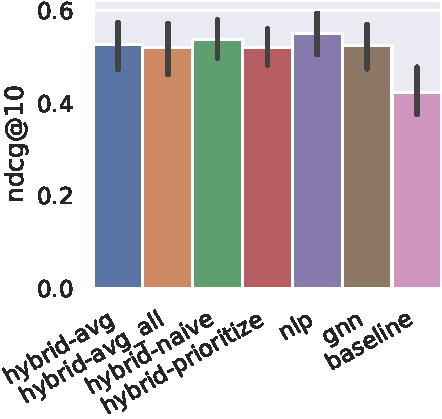
\includegraphics[width=\linewidth]{figures/resultados/7_all-metrics-Decentraland-ndcg@10.pdf}
        \caption{Decentraland}
    \end{subfigure}\hfill\begin{subfigure}{.24\linewidth}
        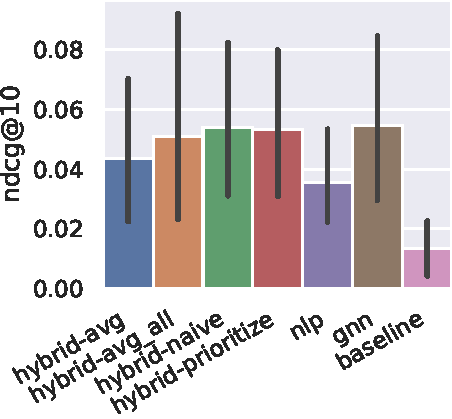
\includegraphics[width=\linewidth]{figures/resultados/7_all-metrics-DEAD FoundationsDAO-ndcg@10.pdf}
        \caption{DEAD Foundations}
        \label{fig:all-results-ndcg-dead_foundation}
    \end{subfigure}\hfill\begin{subfigure}{.24\linewidth}
        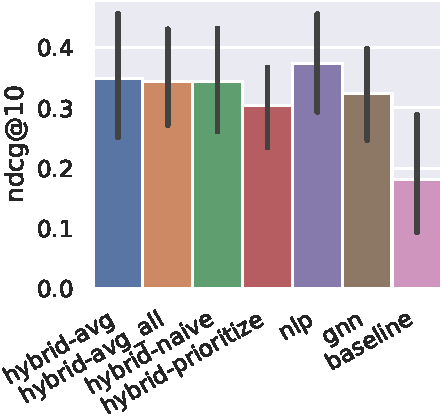
\includegraphics[width=\linewidth]{figures/resultados/7_all-metrics-MetaCartel - MetaCartel Ventures-ndcg@10.pdf}
        \caption{Metacartel}
    \end{subfigure}\hfill\begin{subfigure}{.24\linewidth}
        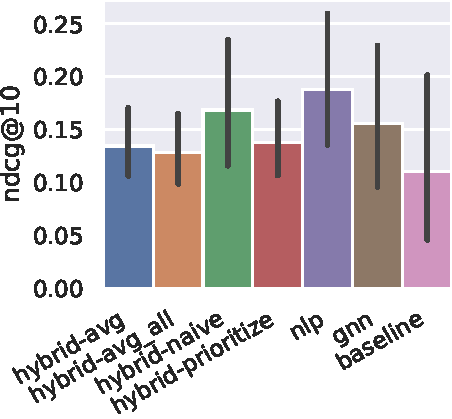
\includegraphics[width=\linewidth]{figures/resultados/7_all-metrics-PancakeSwap-ndcg@10.pdf}
        \caption{PancakeSwap}
    \end{subfigure}
    \caption{Resultados de la métrica ndcg@10 en las organizaciones probadas.}
    \label{fig:all-results-ndcg}
\end{figure}
\begin{figure}[t]
    \centering
    \begin{subfigure}{.24\linewidth}
        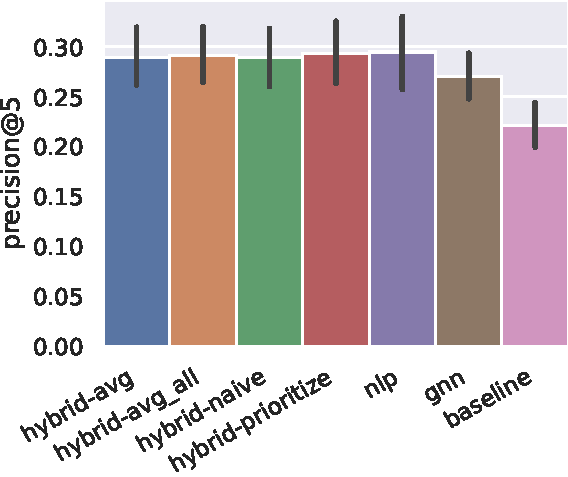
\includegraphics[width=\linewidth]{figures/resultados/7_all-metrics-Decentraland-precision@5.pdf}
        \caption{Decentraland}
    \end{subfigure}\hfill\begin{subfigure}{.24\linewidth}
        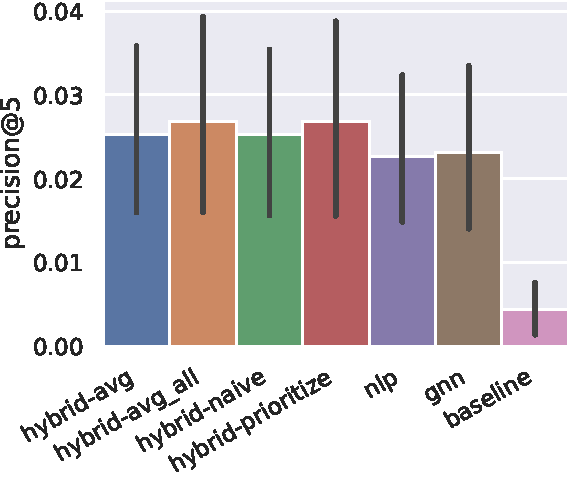
\includegraphics[width=\linewidth]{figures/resultados/7_all-metrics-DEAD FoundationsDAO-precision@5.pdf}
        \caption{DEAD Foundations}
        \label{fig:all-results-precision-dead_foundations}
    \end{subfigure}\hfill\begin{subfigure}{.24\linewidth}
        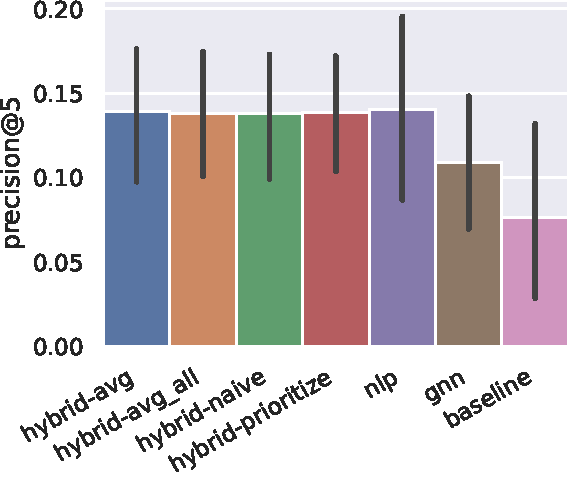
\includegraphics[width=\linewidth]{figures/resultados/7_all-metrics-MetaCartel - MetaCartel Ventures-precision@5.pdf}
        \caption{Metacartel}
    \end{subfigure}\hfill\begin{subfigure}{.24\linewidth}
        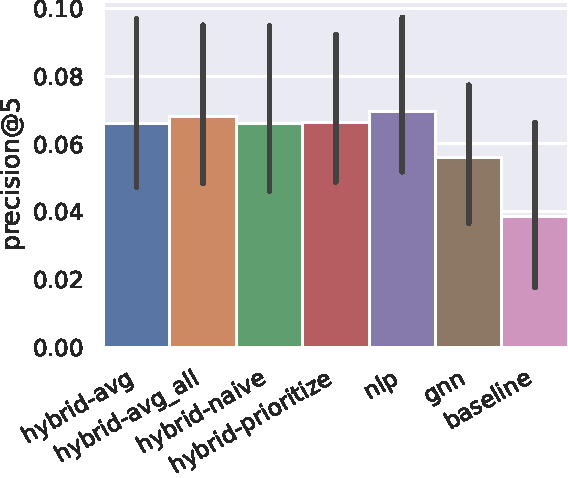
\includegraphics[width=\linewidth]{figures/resultados/7_all-metrics-PancakeSwap-precision@5.pdf}
        \caption{PancakeSwap}
    \end{subfigure}
    \caption{Resultados de la métrica precision@5 en las organizaciones probadas.}
    \label{fig:all-results-precision}
\end{figure}

El modelo GNN, basado en filtrado colaborativo, demuestra el desafío de arranque en frío (\textit{cold-start}) que sufren este tipo de modelos para cada una de las propuestas que se crean continuamente, y que cuentan con pocas interacciones. Como se detalla en la subsección~\ref{subsec:recsys-content}, los sistemas basados en contenido sufren menos dicho problema. Aunque presentan el problema de \textit{cold-start} con usuarios, en este tipo de organizaciones el número de usuarios es relativamente estable.

En cuanto al híbrido, en general logra unos resultados que se sitúan entre el modelo basado en contenido y el basado en filtrado colaborativo. En cuanto a los distintos métodos de fusión de las recomendaciones, las otras organizaciones tienen unas conclusiones similares al caso de Decentraland (véase la subsección~\ref{subsec:implementacion-hybrid}): el método de entrelazado simple parece lograr mejores resultados de \textit{ranking} porque prioriza el PLN, que es el mejor modelo.

La única excepción de entre las organizaciones usadas es DEAD Foundations, en el que el sistema híbrido supera al basado en GNN, que a su vez supera al basado en contenido. 
Esta DAO, además, cuenta con una línea base especialmente baja, y es de hecho la organización con menor densidad ($\simeq2\permil$), como se muestra en la tabla~\ref{tab:4_daos_relevantes}. Este hecho podría indicar que un enfoque híbrido es el camino a seguir para realizar mejores recomendaciones en organizaciones dispersas, que sí que pueden contar con ambos problemas de \textit{cold-start}.

Aunque en todas las organizaciones probadas se supere la linea base, es necesario considerar el contexto específico de cada organización para seleccionar o desarrollar el mejor enfoque de recomendación, analizando su actividad y las características de los usuarios y las propuestas. 
